\documentclass[a4paper]{article}
\usepackage[utf8]{inputenc}
\usepackage[T1]{fontenc}
\usepackage{cite}
\usepackage{graphicx}
\usepackage{hyperref}


\iffalse
1) Le contexte, la problèmatique, les contributions de l’article choisi (2 pages environ)
2) Le plan d’expérience que vous comptez mener, les données que vous comptez utiliser (2 pages max).
\fi

\title{Projet AS : WaveNet}
\author{Seurin Mathieu}

\begin{document}

\maketitle

\section{Contexte : Génération de son}

Le but de WaveNet \cite{DBLP:journals/corr/OordDZSVGKSK16} est de faire de la génération de son brut et plus particulièrement la génération de voix humaine (on verra que WaveNet va plus loin). L'idée est simple, le programme reçoit en entrée un texte, et le but est de faire sortir une voix la plus réalise possible, récitant le texte. Cette tâche s'appelle de la synthèse vocal ou TTS (Text-To-Speech).

Il existe deux concurrents actuellement et c'est avec eux que WaveNet sera comparé. Le premier s'appelle 'concatenative TTS' (méthode par concatenation) et le deuxième 'parametric TTS' (méthode paramétrique). La méthode par concatenation utilise pleins d'enregistrements de voix et les 'colle' bout à bout pour générer le discours mis en entrée. Le processus fonctionne relativemment bien mais il a ses limites. L'enregistrement est coûteux car il faut le faire pour chaque mot (et rajouter un mot nécessite un nouvel enregistrement) et l'enregistrement doit être très precis (même timbre de voix, même vitesse de parole, même volume etc ...). De plus, ajouter une nouvelle voix oblige à ré-enregistrer tout. La deuxième méthode est paramétrique : Au lieu de coller des enregistrements de mots, le discours va être généré par le modèle. Les premiers sont des modèles dits de vocodeur, où on va appliquer plusieurs filtres sur un signal pour simuler l'appareil vocal d'un humain et donc simuler une voix.
Les deuxièmes sont des modèles qui auront appris sur une base de voix humaine (WaveNet rentrent dans cette catégorie, de modèles appris sur de la voix humaine). Classiquement ces modèles sont à base de chaines de Markov.

La problématique est d'obtenir un son de voix qui est le plus naturel possible et avoir des modèles flexibles. Les modèles par concatenation sonnant relativement bien, parfois un peu haché, mais ils ne sont pas du tout flexible. Actuellement les modèles paramétriques sont plus flexible, mais sonne moins naturel que les méthodes par concatenation.
L'objectif de WaveNet est donc de créer un modèle paramétrique flexible et qui soit au moins aussi bon que des modèles par concatenation.

\section{L'approche de WaveNet}

L'approche WaveNet est celle d'un modèle paramétrique, avec base d'apprentissage. Pour le moment, la littérature est centrée sur des modèles RNN et LSTM \cite{DBLP:journals/corr/ZenAEHS16}., mais on trouve également des modèles Markoviens \cite{zen2009statistical}.

L'approche WaveNet est à base de réseaux de neurones convolutifs causaux dilatés. Nous allons expliquer le principe plus en détails.

Le but est de générer un signal d'environ 16000 échantillons à la seconde, chaque échantillon dépendant des échantillons précédents (on verra dans quel mesure).
L'architecture proposée n'est pas à base de RNN mais de réseaux de convolutions causaux, ce qui veut dire que l'output $x_t$ (échantillon $x$ au temps $t$) va être la résultante de filtres de convolution appliqués au $x_k ... x_{t-1}$ avec $k<t$ (voir \autoref{fig:SimpleModel}, où sont utilisées 3 couches de convolution pour illustrer, dans la réalité, il y a bien plus de couches et les filtres sont plus gros)

\begin{figure}[h]
  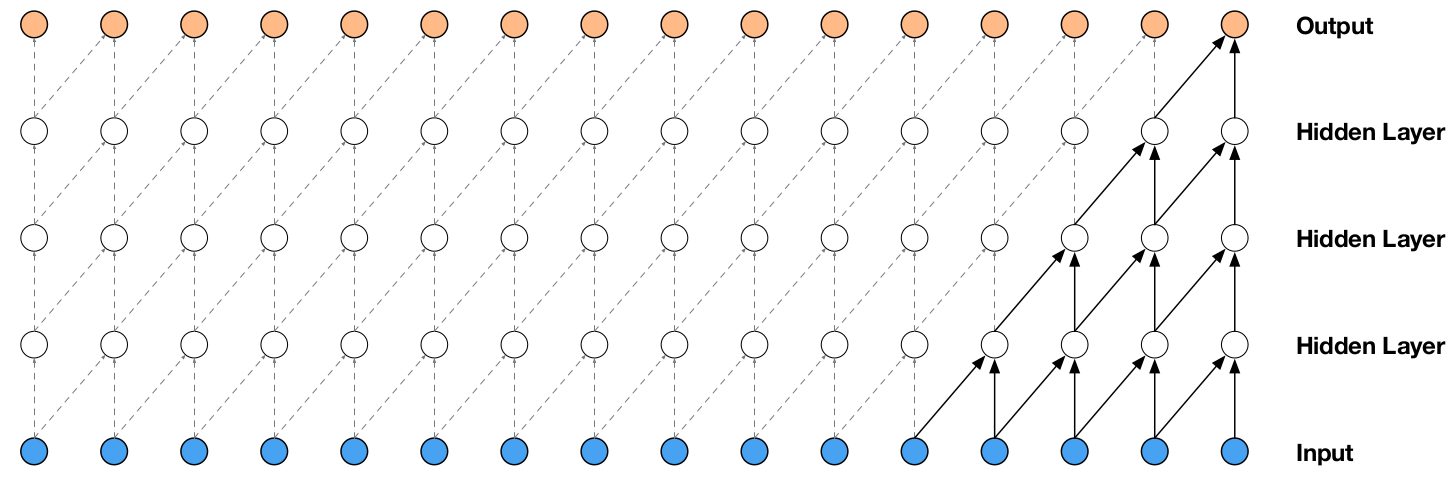
\includegraphics[scale=0.2]{modelSimple.png}
  \caption{\label{fig:SimpleModel} Réseaux de convolutions causaux}
\end{figure}

Le principal problème de cette architecture est qu'elle a besoin d'énormément de couches (combinaisons de plusieurs filtres) et de filtres gros (= qui filtrent beaucoup de pas de temps et qui remonte loin dans le passé), cela pose donc un problème niveau temps/coût de calcul.

Pour remédier au deuxième problème, les auteurs utilisent une structure différente : Les CNN causaux dilatés. Le principe est illustré sur la \autoref{fig:modelDilate}. Le but est d'augmenter la taille des filtres des couches cachées mais sans décupler le nombre de calcul à effectuer. Cela permet aux filtres des couches cachés de récupérer de l'infos de pas de temps plus éloignés.

Plus l'on va dilater un filtre, plus il va capter l'information de pas temps éloignés. Attention, un fitre trop dilaté risque de 'sauter' des pas de temps et d'ignorer les échantillons récents, ce qui n'est pas un comportement voulu.

\begin{figure}[h]
  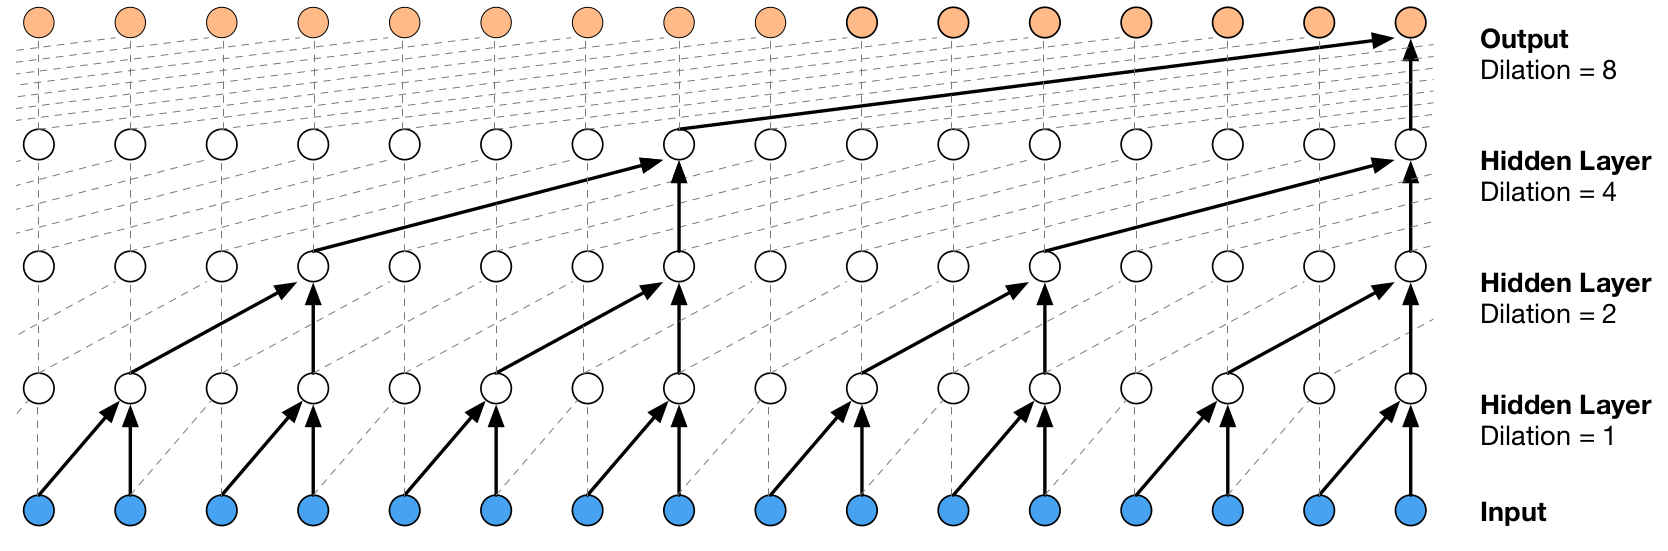
\includegraphics[scale=0.2]{modelDilate.png}
  \caption{\label{fig:modelDilate} Réseaux de convolutions causaux}
\end{figure}

\section{Plan d'expérience}

L'application de WaveNet est évidemment la génération de voix humaine, mais à la fin de l'article, les auteurs montrent que le modèle peut être exploité pour générer d'autres types de sons et plus précisément de la musique. Pour cela, le modèle est légèrement adapté, et ne prend pas de texte en entrée à réciter. Cette approche de génération de musique brute existe déjà avec le modèle GRUV \cite{nayebigruv} qui lui utilise un modèle à base de RNN et de LSTM. Il pourrait être intéressant de comparer les deux sur plusieurs points :


\begin{enumerate}
\item La qualité du son sera le principal critère de comparaison
\item La vitesse d'apprentissage des modèles :
  \begin{enumerate}
  \item Temps de calcul pour une epoch
  \item Temps de convergence global (ou temps pour avoir une qualité de son correct)
  \end{enumerate}
\end{enumerate}

Pour aller plus loin : (Plutôt côté qualité de la musique)
\begin{enumerate}
\item Est-ce que le modèle réutilise des bouts entiers ou arrive à s'en détacher ?
\item Est-ce que des parties sonnent plutôt fausses (ou très dissonantes)
\item Rythmique boiteuse ou très calée ?
\end{enumerate}


L'objectif va être de ré-implémenter WaveNet en torch, car ceci est l'objectif principal du projet, mais également d'utiliser une bibliothèque de RNN et LSTM pour reproduire au mieux GRUV. Les temps d'execution vont être mesurés à la fois pour itérer sur une epoch et de façon plus général, lequel des deux va le plus vite pour obtenir un son d'une qualité correcte.

La partie sur la qualité du son introduit un peu de subjectivité, mais on peut définir des critères de qualité du son assez génériques et objectifs.

\begin{enumerate}
\item Pas de bruit ambiant (grésillements)
\item Pas de coupure de son brusque
\item Pas de gros changements de volume
\end{enumerate}

Après quant à la qualité de la musique en elle-même, cela devient très subjectif (et dépendant du style appris).

\subsection{Données utilisées}

La base d'apprentissage de WaveNet comportait 60h de musique. Le plus simple étant de récupérer des playlists youtube de plusieurs heures, que l'on transformera ensuite. Je commencerai sur un instrument seul (type guitare acoustique). J'ai pour le moment une base d'environ 10h de guitare acoustique seule. Si cela fonctionne à merveille, on pourra tenter des morceaux plus compliqués avec plus d'instruments, j'ai pour cela une base de 12h de musique celtique instrumentale.


\bibliography{rapport29Nov}
\bibliographystyle{apalike}
\end{document}
